% A LaTeX template for MSc Thesis submissions to 
% Politecnico di Milano (PoliMi) - School of Industrial and Information Engineering
%
% S. Bonetti, A. Gruttadauria, G. Mescolini, A. Zingaro
% e-mail: template-tesi-ingind@polimi.it
%
% Last Revision: October 2021
%
% Copyright 2021 Politecnico di Milano, Italy. NC-BY

\documentclass{Configuration_Files/PoliMi3i_thesis}

%------------------------------------------------------------------------------
%	REQUIRED PACKAGES AND  CONFIGURATIONS
%------------------------------------------------------------------------------

% CONFIGURATIONS
\usepackage{parskip} % For paragraph layout
\usepackage{setspace} % For using single or double spacing
\usepackage{emptypage} % To insert empty pages
\usepackage{multicol} % To write in multiple columns (executive summary)
\setlength\columnsep{15pt} % Column separation in executive summary
\setlength\parindent{0pt} % Indentation
\raggedbottom  

% PACKAGES FOR TITLES
\usepackage{titlesec}
% \titlespacing{\section}{left spacing}{before spacing}{after spacing}
\titlespacing{\section}{0pt}{3.3ex}{2ex}
\titlespacing{\subsection}{0pt}{3.3ex}{1.65ex}
\titlespacing{\subsubsection}{0pt}{3.3ex}{1ex}
\usepackage{color}

% PACKAGES FOR LANGUAGE AND FONT
\usepackage[english]{babel} % The document is in English  
\usepackage[utf8]{inputenc} % UTF8 encoding
\usepackage[T1]{fontenc} % Font encoding
\usepackage[11pt]{moresize} % Big fonts

% PACKAGES FOR IMAGES
\usepackage{graphicx}
\usepackage{transparent} % Enables transparent images
\usepackage{eso-pic} % For the background picture on the title page
\usepackage{subfig} % Numbered and caption subfigures using \subfloat.
\usepackage{tikz} % A package for high-quality hand-made figures.
\usetikzlibrary{}
\graphicspath{{./Images/}} % Directory of the images
\usepackage{caption} % Coloured captions
\usepackage{xcolor} % Coloured captions
\usepackage{amsthm,thmtools,xcolor} % Coloured "Theorem"
\usepackage{float}

% STANDARD MATH PACKAGES
\usepackage{amsmath}
\usepackage{amsthm}
\usepackage{amssymb}
\usepackage{amsfonts}
\usepackage{bm}
\usepackage[overload]{empheq} % For braced-style systems of equations.
\usepackage{fix-cm} % To override original LaTeX restrictions on sizes

% PACKAGES FOR TABLES
\usepackage{tabularx}
\usepackage{longtable} % Tables that can span several pages
\usepackage{colortbl}

% PACKAGES FOR ALGORITHMS (PSEUDO-CODE)
\usepackage{algorithm}
\usepackage{algpseudocode}
% PACKAGES FOR REFERENCES & BIBLIOGRAPHY
\usepackage[backend=biber]{biblatex} %Imports biblatex package, specify biber backend
\addbibresource{mimesis.bib}
% PACKAGES FOR REFERENCES & BIBLIOGRAPHY
\usepackage[colorlinks=true,linkcolor=black,anchorcolor=black,citecolor=black,filecolor=black,menucolor=black,runcolor=black,urlcolor=black]{hyperref} % Adds clickable links at references
\usepackage{cleveref}

% OTHER PACKAGES
\usepackage{pdfpages} % To include a pdf file
\usepackage{afterpage}
\usepackage{lipsum} % DUMMY PACKAGE
\usepackage{fancyhdr} % For the headers
\fancyhf{}

% Input of configuration file. Do not change config.tex file unless you really know what you are doing. 
% Set the geometric layout of the document
\usepackage{geometry}
\geometry{
  top=3cm,
  left = 2.0cm,
  right = 2.0cm,
  bottom=2cm,
  headheight= 2cm,
  headsep= 0cm,
}
\raggedbottom

% Create color bluePoli (-> manuale grafica coordinata:  https://www.polimi.it/fileadmin/user_upload/il_Politecnico/grafica-coordinata/2015_05_11_46xy_manuale_grafica_coordinata.pdf)
\definecolor{bluePoli}{cmyk}{0.4,0.1,0,0.4}

% Custom theorem environments
\declaretheoremstyle[
  shaded={rulecolor=bluePoli!20, rulewidth=1pt, bgcolor=bluePoli!5},
  headfont=\color{bluePoli}\normalfont\bfseries,
  bodyfont=\color{black}\normalfont,
]{colored}

\captionsetup[figure]{labelfont={color=bluePoli}} % Set colour of the captions
\captionsetup[table]{labelfont={color=bluePoli}} % Set colour of the captions
\captionsetup[algorithm]{labelfont={color=bluePoli}} % Set colour of the captions

\theoremstyle{colored}
\newtheorem{theorem}{Theorem}[section]
\newtheorem{proposition}{Proposition}[section]
\newtheorem{definition}{Definition}[section]
\newtheorem*{remark}{Remark}
\newtheorem{lemma}{Lemma}[section]

% Enhances the features of the standard "table" and "tabular" environments.
\newcommand\T{\rule{0pt}{2.6ex}}
\newcommand\B{\rule[-1.2ex]{0pt}{0pt}}

% Algorithm description
\newcounter{algsubstate}
\renewcommand{\thealgsubstate}{\alph{algsubstate}}
\newenvironment{algsubstates}{
    \setcounter{algsubstate}{0}%
    \renewcommand{\STATE}{%
    \stepcounter{algsubstate}%
    \Statex {\small\thealgsubstate:}\space}
    }{}

% Custom theorem environment
\newcolumntype{L}[1]{>{\raggedright\let\newline\\\arraybackslash\hspace{0pt}}m{#1}}
\newcolumntype{C}[1]{>{\centering\let\newline\\\arraybackslash\hspace{0pt}}m{#1}}
\newcolumntype{R}[1]{>{\raggedleft\let\newline\\\arraybackslash\hspace{0pt}}m{#1}}

% Custom itemize environment
\setlist[itemize,1]{label=$\bullet$}
\setlist[itemize,2]{label=$\circ$}
\setlist[itemize,3]{label=$-$}
\setlist{nosep}

% Set separation of columns
\setlength{\columnsep}{30pt}

% Create command for background pic
\newcommand\BackgroundPic{% Adding background picture
	\put(230,358){
		\parbox[b][\paperheight]{\paperwidth}{%
			\vfill
			\centering
			\transparent{0.2}
			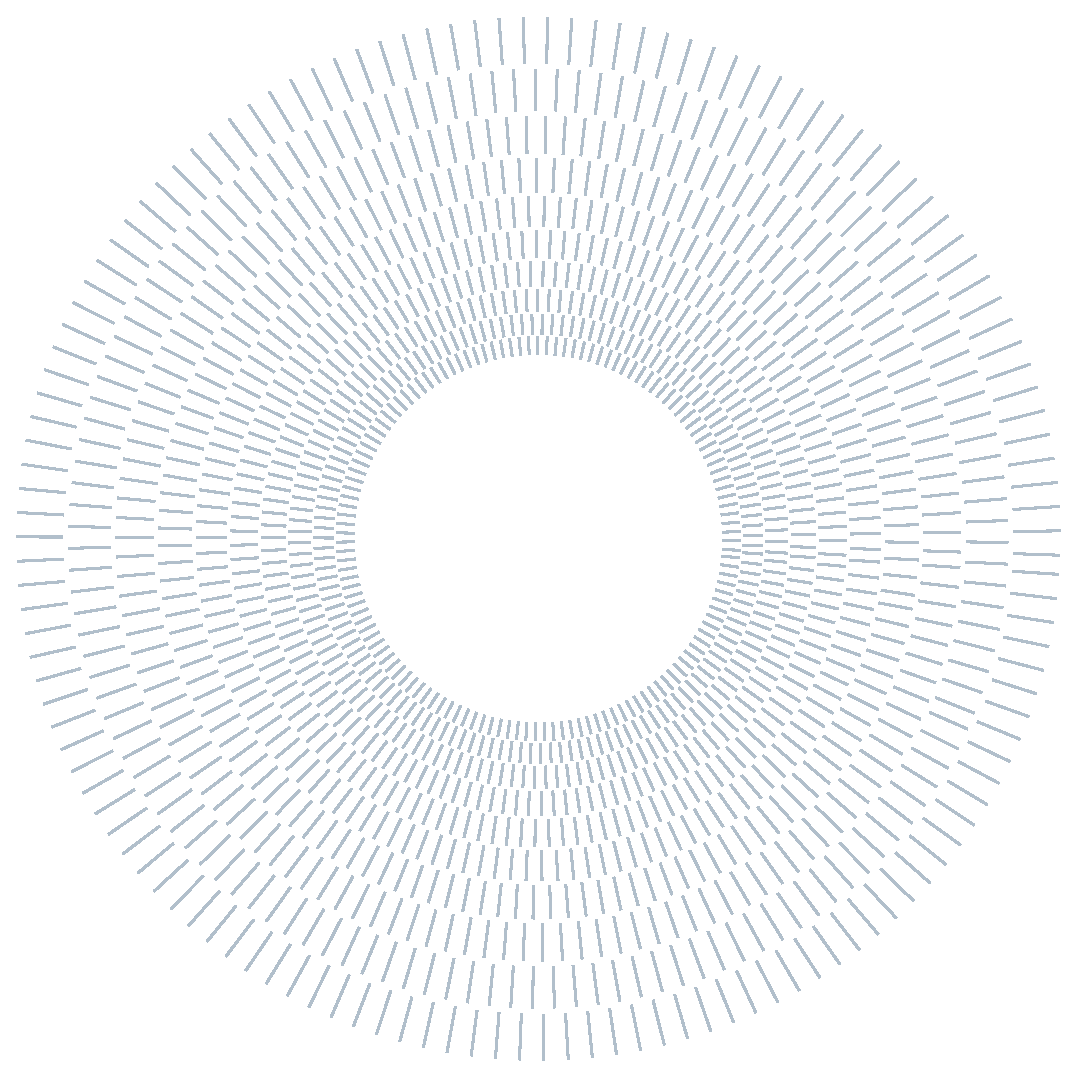
\includegraphics[width=0.8\paperwidth]{raggiera_polimi.eps}%
			\vfill
}}}

% Set indentation
%\setlength\parindent{0pt}

% Custom title commands
\titleformat{\section}
{\color{bluePoli}\normalfont\Large\bfseries}
{\color{bluePoli}\thesection.}{1em}{}
\titlespacing*{\section}
{0pt}{2ex}{1ex}

\titleformat{\subsection}
{\color{bluePoli}\normalfont\large\bfseries}
{\color{bluePoli}\thesubsection.}{1em}{}
\titlespacing*{\subsection}
{0pt}{2ex}{1ex}

\titleformat{\subsubsection}
{\color{bluePoli}\normalfont\normalsize\bfseries}
{\color{bluePoli}\thesubsubsection.}{1em}{}
\titlespacing*{\subsubsection}
{0pt}{2ex}{1ex}

% Custom headers and footers
\pagestyle{fancy}
\fancyhf{}

\fancyfoot{}
\fancyfoot[C]{\thepage} % page
\renewcommand{\headrulewidth}{0mm} % headrule width
\renewcommand{\footrulewidth}{0mm} % footrule width

\makeatletter
\patchcmd{\headrule}{\hrule}{\color{black}\hrule}{}{} % headrule
\patchcmd{\footrule}{\hrule}{\color{black}\hrule}{}{} % footrule
\makeatother

% -> Create the header
\chead[C]{
\centering
\begin{tcolorbox}[arc=0pt, boxrule=0pt, colback=bluePoli!60, width=\textwidth, colupper=white]
    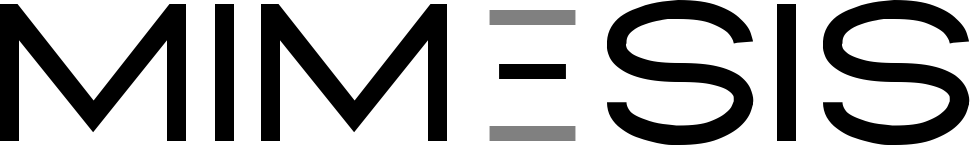
\includegraphics[width=0.2\textwidth]{mimesis.png}
\end{tcolorbox}
}


%----------------------------------------------------------------------------
%	NEW COMMANDS DEFINED
%----------------------------------------------------------------------------

% EXAMPLES OF NEW COMMANDS
\newcommand{\bea}{\begin{eqnarray}} % Shortcut for equation arrays
\newcommand{\eea}{\end{eqnarray}}
\newcommand{\e}[1]{\times 10^{#1}}  % Powers of 10 notation

%----------------------------------------------------------------------------
%	ADD YOUR PACKAGES (be careful of package interaction)
%----------------------------------------------------------------------------

%----------------------------------------------------------------------------
%	ADD YOUR DEFINITIONS AND COMMANDS (be careful of existing commands)
%----------------------------------------------------------------------------
\newcommand*{\oldepsilon}{\epsilon}
\renewcommand*{\epsilon}{\varepsilon}
\DeclareMathOperator*{\esssup}{ess\,sup}
\DeclareMathOperator*{\argmax}{arg\,max}
\DeclareMathOperator*{\argmin}{arg\,min}
%----------------------------------------------------------------------------
%	BEGIN OF YOUR DOCUMENT
%----------------------------------------------------------------------------

\begin{document}

\fancypagestyle{plain}{%
\fancyhf{} % Clear all header and footer fields
\fancyhead[RO,RE]{\thepage} %RO=right odd, RE=right even
\renewcommand{\headrulewidth}{0pt}
\renewcommand{\footrulewidth}{0pt}}

%----------------------------------------------------------------------------
%	TITLE PAGE
%----------------------------------------------------------------------------

\pagestyle{empty} % No page numbers
\frontmatter % Use roman page numbering style (i, ii, iii, iv...) for the preamble pages

\puttitle{
	title=Neural Modes, % Title of the thesis
	name=Andrea Bonifacio, % Author Name and Surname
	course=Mathematical Engineering - Ingegneria Matematica, % Study Programme (in Italian)
	ID  = 217658,  % Student ID number (numero di matricola)
	advisor= Prof. Stefano Pagani, % Supervisor name
	coadvisor={Stéphane Cotin}, % Co-Supervisor name, remove this line if there is none
	academicyear={2024-25},  % Academic Year
} % These info will be put into your Title page 

%----------------------------------------------------------------------------
%	PREAMBLE PAGES: ABSTRACT (inglese e italiano), EXECUTIVE SUMMARY
%----------------------------------------------------------------------------
\startpreamble
\setcounter{page}{1} % Set page counter to 1

% ABSTRACT IN ENGLISH
\chapter*{Abstract} 
Here goes the Abstract in English of your thesis followed by a list of keywords.
The Abstract is a concise summary of the content of the thesis (single page of text)
and a guide to the most important contributions included in your thesis.
The Abstract is the very last thing you write.
It should be a self-contained text and should be clear to someone who hasn't (yet) read the whole manuscript.
The Abstract should contain the answers to the main scientific questions that have been addressed in your thesis.
It needs to summarize the adopted motivations and the adopted methodological approach as well as the findings of your work and their relevance and impact.
The Abstract is the part appearing in the record of your thesis inside POLITesi,
the Digital Archive of PhD and Master Theses (Laurea Magistrale) of Politecnico di Milano.
The Abstract will be followed by a list of four to six keywords.
Keywords are a tool to help indexers and search engines to find relevant documents.
To be relevant and effective, keywords must be chosen carefully.
They should represent the content of your work and be specific to your field or sub-field.
Keywords may be a single word or two to four words. 
\\
\\
\textbf{Keywords:} here, the keywords, of your thesis % Keywords

% ABSTRACT IN ITALIAN
\chapter*{Abstract in lingua italiana}
Qui va l'Abstract in lingua italiana della tesi seguito dalla lista di parole chiave.
\\
\\
\textbf{Parole chiave:} qui, vanno, le parole chiave, della tesi % Keywords (italian)

%----------------------------------------------------------------------------
%	LIST OF CONTENTS/FIGURES/TABLES/SYMBOLS
%----------------------------------------------------------------------------

% TABLE OF CONTENTS
\thispagestyle{empty}
\tableofcontents % Table of contents 
\thispagestyle{empty}
\cleardoublepage

%-------------------------------------------------------------------------
%	THESIS MAIN TEXT
%-------------------------------------------------------------------------
% In the main text of your thesis you can write the chapters in two different ways:
%
%(1) As presented in this template you can write:
%    \chapter{Title of the chapter}
%    *body of the chapter*
%
%(2) You can write your chapter in a separated .tex file and then include it in the main file with the following command:
%    \chapter{Title of the chapter}
%    \input{chapter_file.tex}
%
% Especially for long thesis, we recommend you the second option.

\addtocontents{toc}{\vspace{2em}} % Add a gap in the Contents, for aesthetics
\mainmatter % Begin numeric (1,2,3...) page numbering

% --------------------------------------------------------------------------
% NUMBERED CHAPTERS % Regular chapters following
% --------------------------------------------------------------------------
\chapter*{Introduction}
\section{Introduction}

Numerical simulations play a critical role in a wide array of scientific and engineering applications, providing insights into the behavior of physical systems under various conditions. Among the most prominent techniques for performing such simulations is Finite Element Modeling (FEM). FEM discretizes a continuous domain into a mesh of finite elements, allowing for the approximation of solutions to complex partial differential equations (PDEs). However, one significant drawback of FEM is its computational intensity, especially when high resolution is required for accurate results. This research aims to explore the potential of Deep Learning (DL) techniques to accelerate FEM simulations, focusing specifically on the deformation of objects subjected to external forces.

The deformation of an object under an applied force is directly tied to the object's discretization. In FEM, the object is represented by a mesh, where the resolution of the mesh—i.e., the size and number of elements—clearly impacts the accuracy and computational cost of the simulation. High-resolution meshes can capture fine details of deformation, leading to more accurate simulations, but they are computationally expensive and time-consuming. 

The main goal of this work is to study the efficacy of a method that combines both Finite Element Modeling (FEM) and DL to obtain a realistic simulation of an object in a fraction of the time that would be required by a traditional FEM simulation. The idea is to, somehow, train a DL model to have inside the information given by the refined discretization and pass them on a coarser discretization.

The idea of using DL techniques to solve scientific problem is not new. Thanks to the rise of new frameworks and libraries, such as TensorFlow and PyTorch, it is now possible to train very complex models on large datasets in a reasonable amount of time. For the problem at hand, a lot of different approaches can be found in the existing literature: a lot of them are based on the idea that the deep learning model should predict the whole dynamic of the system, for example MeshGraphNet \cite{pfaffLearningMeshBasedSimulation2021a} or its multiscale version \cite{fortunatoMultiScaleMeshGraphNets2022}, but these are just two examples of the many possible approaches \cite{jiangMeshfreeFlowNetPhysicsConstrainedDeep2020}, \cite{djeumouNeuralNetworksPhysicsInformed2022}, \cite{hanPredictingPhysicsMeshreduced2022a}. Other methods rely on solving a time independent problem, using various architectures, such as PINNs \cite{djeumouNeuralNetworksPhysicsInformed2022} or GNNs \cite{gaoPhysicsinformedGraphNeural2022}. The proposed method falls into the second category, as it will be explained in the following sections.

One interesting solution is given by \cite{Wang_Du_Coros_Thomaszewski_2024}, where the authors extend the concept of linear modes and modal dynamics \cite{Pentland_Williams_1989} to be able to handle larger deformations. The key idea is to obtain a linear approximation of the deformation, then train a network to minimize the energy of the system, so that for every modal coordinate, the network will learn a non-linear correction, effectively learning a series of non-linear modes. This allows for faster simulations by exploiting subspace dynamics, where the simulation is performed in a reduced space to ease computational costs. The authors show that 



\chapter{Mathematical Model}
\label{ch:chapter_one}%
\section{Problem setting}
In this section will be outlined a mathematical description of the problem. It will be divided in the two case under study: the static case and the dynamic case.

\subsection{Static case}
The static case is the simplest one. In this case we have a domain $\Omega \subset \mathbb{R}^d$ with $d=2,3$ and a force $f$ acting on it. A Lagrangian description of the problem is considered, where the material coordinates are given by the vector $\bm{X}$ and the deformed state of the solid is given by
\begin{equation}
    \bm{x} = \bm{X} + \bm{u}
\label{eq:deformation}
\end{equation}
where $\bm{u}$ is the displacement field. The model used to describe the linear relation between the stress tensor $\bm{\sigma} \in \mathbb{R}^{3\times 3}$ and the strain tensor $\bm{\varepsilon} \in \mathbb{R}^{3\times 3}$ is the linear elasticity model, which is given by
\begin{equation}
    \bm{\sigma} = \bm{C} : \bm{\varepsilon}
\label{eq:linear_elasticity}
\end{equation}
where $\bm{C}$ is the stiffness tensor. The strain tensor is given by 
\begin{equation}
    \bm{\varepsilon} = \frac{1}{2} \left( \nabla \bm{u} + (\nabla \bm{u})^T \right)
\label{eq:strain_tensor}
\end{equation}
and the stress tensor is given by
\begin{equation}
    \bm{\sigma} =  2 \mu \bm{\varepsilon} + \lambda \text{tr}(\bm{\varepsilon}) \bm{I}
\label{eq:stress_tensor}
\end{equation}
where $\mu$ is the shear modulus, $\lambda$ is the Lamé parameter and $\bm{I}$ is the identity matrix. The shear modulus and the Lamé parameter are related to the Young's modulus $E$ and the Poisson's ratio $\nu$ by the relations
\begin{equation}
    \mu = \frac{E}{2(1+\nu)}
\end{equation}
and
\begin{equation}
    \lambda = \frac{E\nu}{(1+\nu)(1-2\nu)}
\end{equation}
The boundary \( \partial \Omega \) is divided in two parts: the Dirichlet boundary \( \Gamma_D \) and the Neumann boundary \( \Gamma_N \), where \(\Gamma_D \cup \Gamma_N = \partial \Omega \) and \(\Gamma_D \cap \Gamma_N = \emptyset \). The imposition of the Dirichlet boundary conditions is given by
\begin{equation}
    \bm{u} = \bm{u}_D \quad \text{on} \quad \Gamma_D
\end{equation}
and the imposition of the Neumann boundary conditions is given by
\begin{equation}
    \bm{\sigma} \cdot \bm{n} = \bm{t} \quad \text{on} \quad \Gamma_N
\end{equation}
where \( \bm{n} \) is the outward unit normal to the boundary and \( \bm{t} \) is the traction vector. 

\chapter{Chapter two}
\label{ch:chapter_two}%
\section{Neural Networks}
\label{sec:neural_network}

In this section, a brief outline of the neural network architectures used in this work is given, with particular emphasis on the Neural Modes approach for simulating deformable objects. It will explain how neural networks work in general and specific details about the architectures employed.

\subsection{Neural Network Basics}

A neural network is a mathematical model that achieves statistical generalization drawing inspiration from the human brain. It is possible to define it as a function that maps an input to an output, given a set of parameters \( \bm{\theta} \). The function \( \hat{y} = f(\bm{x}; \bm{\theta}) \) is obtained by composing a series of functions \( f_i \) called layers, where each layer is defined as
\begin{equation}
    f_i = \sigma(W_i f_{i-1} + b_i)
\end{equation}
where \( W_i \) is the weight matrix, \( b_i \) is the bias vector and \( \sigma \) is the activation function. The activation function is a non-linear function that allows the network to learn complex patterns in the data. 

A neural network exists in function of a dataset \( \mathcal{D} = \{(\bm{x}_i, \bm{y}_i)\}_{i=1}^N \), where \( \bm{x}_i \) is the input and \( \bm{y}_i \) is the output. The final goal is to find the set of parameters \( \bm{\theta} \) that minimizes the loss function \( \mathcal{L} \), defined as some metric of the difference between the predicted output and the true output. The loss function:
\begin{equation}
    \mathcal{L} = \frac{1}{N} \sum_{i=1}^N L(f(\bm{x}_i; \bm{\theta}), \bm{y}_i)
\end{equation}
where \( L \) is the loss function, which can be various metrics. The loss function is minimized using an optimization algorithm, so that the objective is to find
\begin{equation}
    \bm{\theta}^* = \argmin_{\bm{\theta}} \mathcal{L}
\end{equation}
which is the best set of parameters that minimizes the loss function.

The full algorithm is the following one:
\begin{algorithm} 
    \caption{Training of a neural network}
    \begin{algorithmic}
        \State Initialize the parameters \( \bm{\theta} \)
        \While{epoch < max\_epochs}
            \For{mini-batch in dataset}
                \State Perform forward pass computing \( f(\bm{x}; \bm{\theta}) \)
                \State Compute the loss function \( \mathcal{L}(f(\bm{x}; \bm{\theta}), \bm{y}) \)
                \State Perform backward pass computing the gradients of the loss function
                \State Update the parameters using the gradients
            \EndFor
        \EndWhile
    \end{algorithmic}
\end{algorithm}

\subsection{Neural Network Architectures}
In this work, we employ a deep feedforward neural network specifically designed for learning nonlinear deformation modes. This architecture builds upon traditional fully connected neural networks but is adapted for the specific task of capturing nonlinear corrections to linear modal displacements.

\subsubsection{Neural Modes Architecture}
The Neural Modes architecture is designed to learn nonlinear corrections to linear deformation modes for Neo-Hookean materials. It consists of a feedforward neural network where:

\begin{itemize}
    \item The input is a modal coordinate vector \( \bm{z} \in \mathbb{R}^m \), where $m$ is the number of modal coordinates.
    \item The output is a nonlinear correction to the displacement field \( \bm{y} \in \mathbb{R}^n \), where $n$ is the total number of degrees of freedom in the mesh.
\end{itemize}

The network learns to map from the reduced modal space to full-dimensional correction vectors that improve the accuracy of the linear modal approximation. This architecture can be visualized as:

\begin{figure}
    \centering
    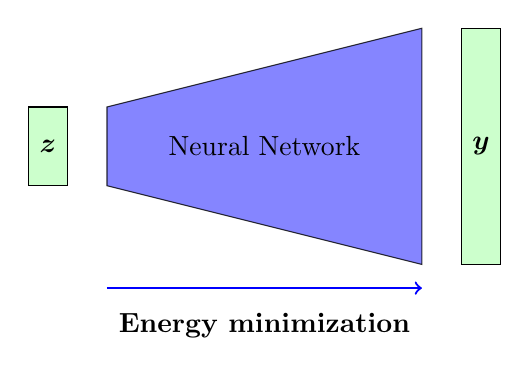
\begin{tikzpicture}
        % Modal coordinate (z)
        \draw[fill=green!20] (-3, 1) rectangle (-2.5,2);
        \node at (-2.75, 1.5) {$\bm{z}$}; % Label inside the rectangle
        
        % Displacement (u)
        \draw[fill=green!20] (2.5,0) rectangle (3,3);
        \node at (2.75, 1.5) {$\bm{y}$}; % Label inside the rectangle
        
        % Energy loss transition
        \draw[fill=blue!60,opacity=0.8] (-2,1) -- (2,-0) -- (2,3) -- (-2,2) -- cycle;
        \node at (0,1.5) {Neural Network};
        \node[below] at (0,-0.5) {\textbf{Energy minimization}};
        
        % Energy loss arrow
        \draw[thick,blue,->] (-2,-0.3) -- (2,-0.3);
    
    \end{tikzpicture}
    \caption{Neural Modes architecture for learning nonlinear deformation corrections}
    \label{fig:neural_modes_arch}
\end{figure}

\subsubsection{Training the Neural Modes}
The training process for the Neural Modes network is based on minimizing a combination of physics-based losses, rather than simply minimizing the prediction error against ground truth data. The key losses used in training are:

\begin{enumerate}
    \item \textbf{Energy Loss}: Minimizes the internal strain energy of the deformed configuration $E(\bm{X} + \bm{l} + \bm{y})$, where $\bm{X}$ is the rest position, $\bm{l}$ is the linear mode displacement given by $\bm{z}$, and $\bm{y}$ is the nonlinear correction.
    
    \item \textbf{Orthogonality Loss}: Ensures that the nonlinear correction is orthogonal to the linear mode space: $\bm{y}^T \bm{l} = 0$.
    
\end{enumerate}

The total loss function is a weighted sum of these individual losses:
\begin{equation}
    \text{Loss} = \text{Energy Loss} + \lambda_1 \text{Orthogonality Loss} + \lambda_2 \text{Origin Loss}
\end{equation}
where $\lambda_1$ and $\lambda_2$ are weight parameters that balance the importance of each loss term.

During the training process, it was observed that the network had the tendency to learn a correction when given \(z = 0\) (i.e., the rest position), and that was not intended, because the rest position should not have any correction, meaning that the model prediction should be zero. To avoid this, the network was designed to have zero bias, so that its output was centered at the origin.

\subsubsection{Dynamic Simulation with Neural Modes}
For dynamic simulations, the Neural Modes framework solves an optimization problem at each time step. Given the current and previous displacement states $\bm{u}_n$ and $\bm{u}_{n-1}$, the modal coordinates for the next time step $\bm{z}_{n+1}$ are computed by:
\begin{equation}
    \bm{z}_{n+1} = \underset{\bm{z}}{\argmin} \frac{1}{2h^2} \|\bm{n}(\bm{z}) - 2\bm{u}_n + \bm{u}_{n-1}\|_{\bm{M}}^2 + E(\bm{n}(\bm{z}))
\end{equation}
where $\bm{n}(\bm{z})$ represents the complete displacement field (linear modes plus nonlinear correction), $h$ is the time step, $\bm{M}$ is the mass matrix, and $E(\cdot)$ is the internal energy of the configuration. This optimization problem is typically solved using the L-BFGS-B algorithm.

One challenge with this approach is that the optimization problem does not explicitly account for external forces. The network learns to minimize internal energy but lacks direct information about external forces that may be applied during simulation. This limitation can affect the accuracy of dynamic simulations, particularly for large deformations or complex loading conditions.

\subsection{Extensions and Improvements}
A possible extension to the Neural Modes approach is to incorporate information about external forces directly into the network. This could be achieved by learning a mapping $\Phi: \mathbb{R}^m \rightarrow \mathbb{R}^n$ that relates modal coordinates $\bm{z}$ to the corresponding external forces $\hat{\bm{f}}$ that would produce such deformation. This additional network could be trained on a dataset of deformations and corresponding external forces, and then integrated into the dynamic simulation process to improve accuracy.

The objective function for dynamic simulation could then be extended to:
\begin{equation}
    \bm{z}_{n+1} = \underset{\bm{z}}{\argmin} \frac{1}{2h^2} \|\bm{n}(\bm{z}) - 2\bm{u}_n + \bm{u}_{n-1}\|_{\bm{M}}^2 + E(\bm{n}(\bm{z})) + \text{F}(\bm{z}, \bm{f})
\end{equation}
where $\text{F}(\bm{z}, \bm{f})$ is a term that accounts for the external forces acting on the system.



\chapter*{Acknowledgements}

\section{Use of copyrighted material}

Each student is responsible for obtaining copyright permissions, if necessary, to include published material in the thesis.
This applies typically to third-party material published by someone else.

\section{Plagiarism}

You have to be sure to respect the rules on Copyright and avoid an involuntary plagiarism.
It is allowed to take other persons' ideas only if the author and his original work are clearly mentioned.
As stated in the Code of Ethics and Conduct, Politecnico di Milano \textit{promotes the integrity of research,
condemns manipulation and the infringement of intellectual property}, and gives opportunity to all those
who carry out research activities to have an adequate training on ethical conduct and integrity while doing research.
To be sure to respect the copyright rules, read the guides on Copyright legislation and citation styles available
at:
\begin{verbatim}
https://www.biblio.polimi.it/en/tools/courses-and-tutorials
\end{verbatim}
You can also attend the courses which are periodically organized on "Bibliographic citations and bibliography management".

\section{Bibliography and citations}
Your thesis must contain a suitable Bibliography which lists all the sources consulted on developing the work.
The list of references is placed at the end of the manuscript after the chapter containing the conclusions.
We suggest to use the BibTeX package and save the bibliographic references  in the file \verb|Thesis_bibliography.bib|.
This is indeed a database containing all the information about the references. To cite in your manuscript, use the \verb|\cite{}| command as follows:
\\
\textit{Here is how you cite bibliography entries: \cite{knuth74}, or multiple ones at once: \cite{knuth92,lamport94}}.
\\
The bibliography and list of references are generated automatically by running BibTeX \cite{bibtex}.

\chapter{Conclusions and future developments}
\label{ch:conclusions}%
A final chapter containing the main conclusions of your research/study
and possible future developments of your work have to be inserted in this chapter.

%-------------------------------------------------------------------------
%	BIBLIOGRAPHY
%-------------------------------------------------------------------------

\addtocontents{toc}{\vspace{2em}} % Add a gap in the Contents, for aesthetics

%-------------------------------------------------------------------------
%	APPENDICES
%-------------------------------------------------------------------------

\cleardoublepage
\addtocontents{toc}{\vspace{2em}} % Add a gap in the Contents, for aesthetics
\appendix
\chapter{Appendix A}
If you need to include an appendix to support the research in your thesis, you can place it at the end of the manuscript.
An appendix contains supplementary material (figures, tables, data, codes, mathematical proofs, surveys, \dots)
which supplement the main results contained in the previous chapters.

\chapter{Appendix B}
It may be necessary to include another appendix to better organize the presentation of supplementary material.


% LIST OF FIGURES
\listoffigures

% LIST OF TABLES
\listoftables

% LIST OF SYMBOLS
% Write out the List of Symbols in this page
\chapter*{List of Symbols} % You have to include a chapter for your list of symbols (
\begin{table}[H]
    \centering
    \begin{tabular}{lll}
        \textbf{Variable} & \textbf{Description} & \textbf{SI unit} \\\hline\\[-9px]
        $\bm{u}$ & solid displacement & m \\[2px]
        $\bm{u}_f$ & fluid displacement & m \\[2px]
    \end{tabular}
\end{table}

% ACKNOWLEDGEMENTS
\chapter*{Acknowledgements}
Here you might want to acknowledge someone.

\cleardoublepage

\end{document}
